\section{Background}
In this section, we give the necessary backgrounds for buddy memory allocation algorithms and Isabelle/HOL theorem prover.

\subsection{Buddy Allocation Algorithms}
Buddy allocation algorithms consist of two main operations: allocation and deallocation of memory blocks. It uses multilevel free linked-list to manage free blocks. All free blocks with same size are linked in the same level in multilevel list. With this list, it is easy to find a free block in requested size if one is available. If one is available, it is directly picked from the head of list in this level. If not, allocation operation searches for the first no-empty free list for blocks, whose size is bigger than requested size. Then, one block which is picked from this no-empty free list is split. It is divided into two smaller blocks, and each smaller block becomes an unique buddy to the other. If the size of smaller block is still too large, one of the two smaller blocks is split again. The split process stops until one block meeting requested size. Then one of the available blocks is returned to the requesting applications. At the same time, this block is marked as occupied in multilevel free bitmap, which is another important structure managing the usage state of each block.

When a block is deallocated, the algorithms check whether the block can be merged. A split block can only be merged with its unique buddy block, which then reforms the larger block they were split from. Among this process, the algorithms search multilevel free bitmap to quickly check if blocks belonging to the same parent are free, in order to decide whether to merge these blocks into one block. With this way, buddy memory system has small external fragmentation. Fig. \ref{fig3} describes a moment in memory system using multilevel free linked-list and multilevel free bitmap.

\begin{figure*}[htbp]
	\centering
	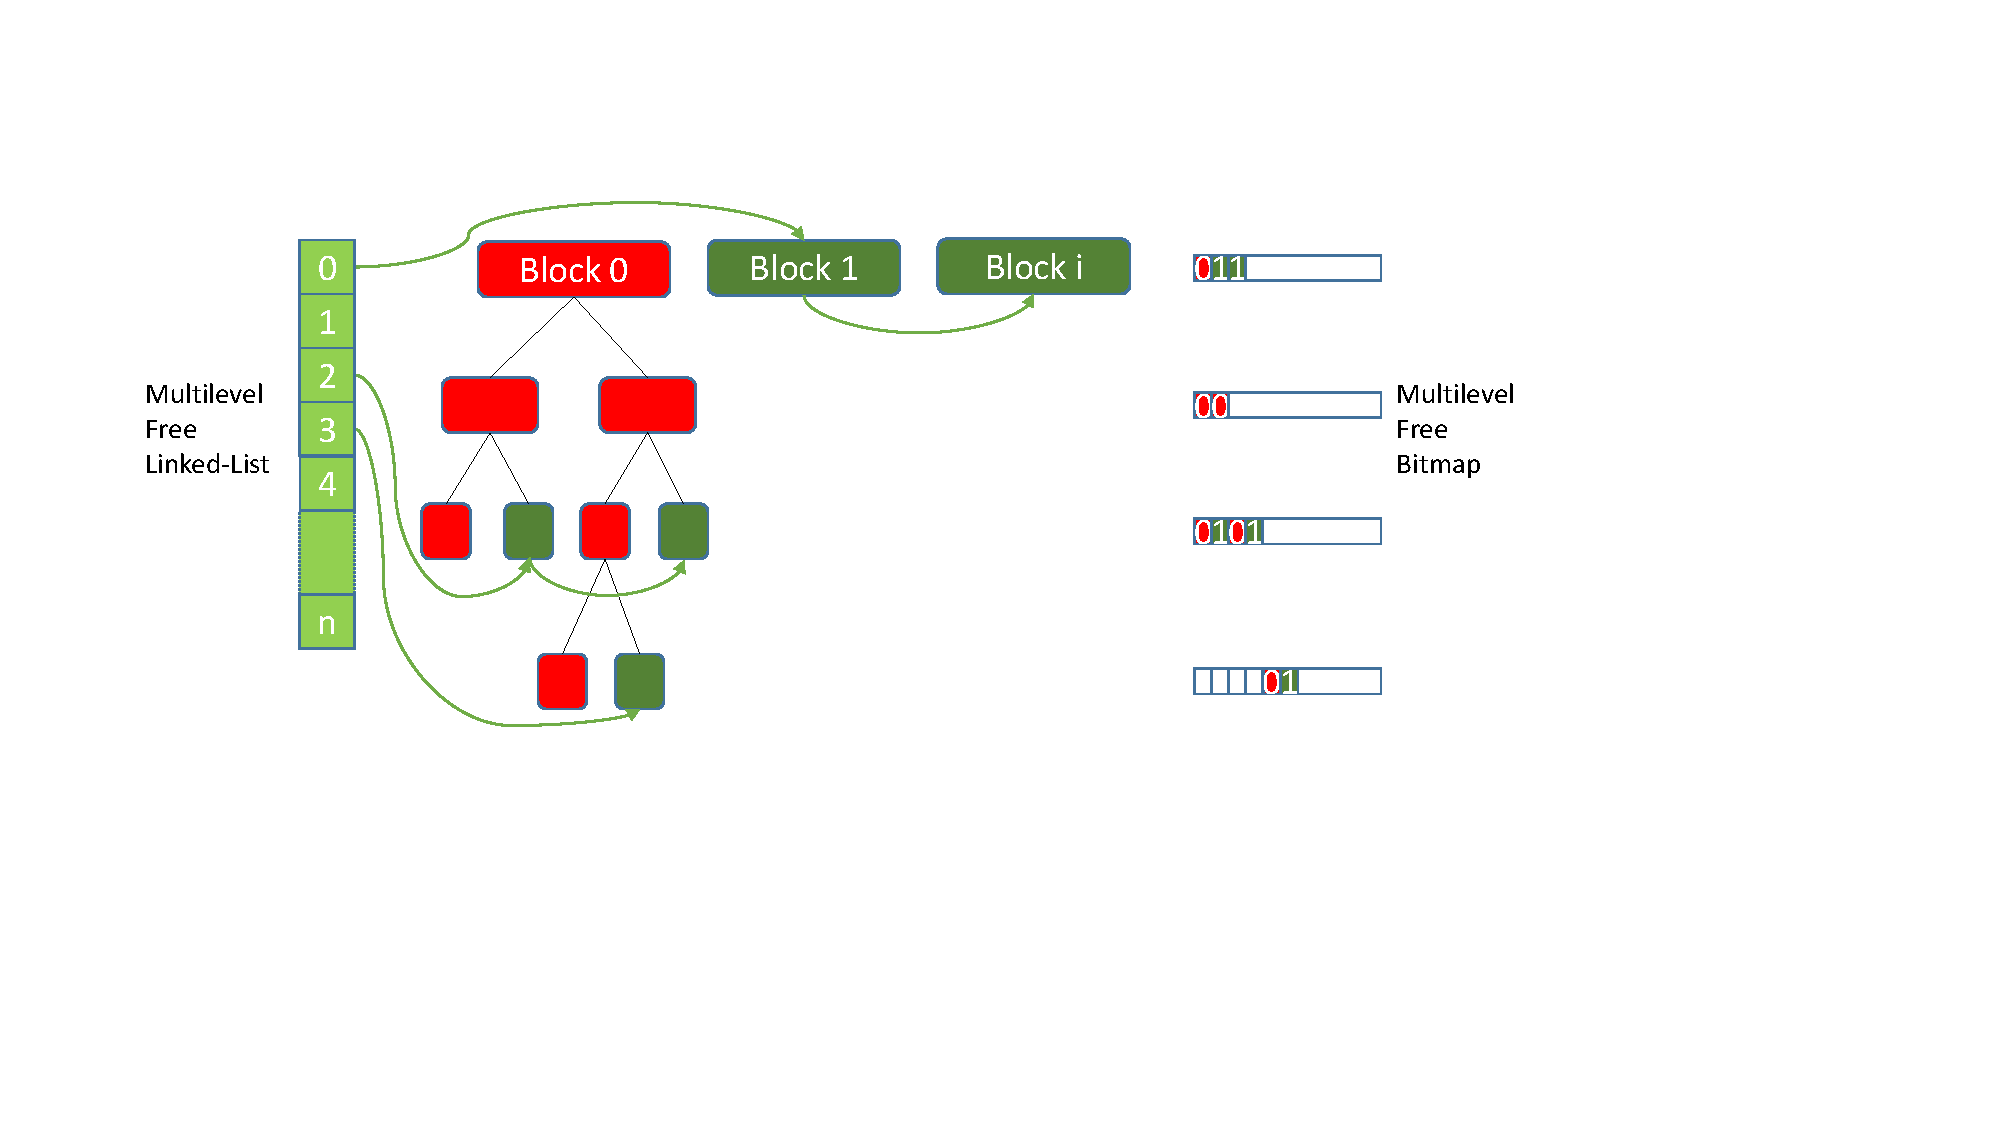
\includegraphics[width=1\textwidth]{fig3.pdf}
	\caption{Structures in Buddy Allocation Algorithms}
	\label{fig3}
\end{figure*}

\subsection{Isabelle/HOL}
We use \correct{interactive theorem prover Isabelle/HOL}{the Isabelle/HOL interactive theorem prover}~\cite{reg_Isabelle/HOL} to conduct the specification and verification of the memory management. Isabelle/HOL is a higher order logic theorem prover, using a typed lambda calculus-like functional language for specifications.

Isabelle/HOL includes a specification for simple common types such as naturals (\emph{nat}), integers (\emph{int}) and booleans (\emph{bool}). It also specifies some composed data types like tuples, records, lists and sets that are parametrized with other types. Isabelle provides the interface \emph{datatype} for the creation of user defined types based on type constructors. 

Isabelle provides functions on predefined types to access their members or to provide additional operations over them. In the following we describe those functions and types that we use along this work. A tuple is denoted as (\emph{$t_1$} $\times$ \emph{$t_2$}), projection functions \emph{fst} and \emph{snd} respectively return elements $t_1$ and $t_2$. Lists are defined as a datatype with an empty construct denoted with \emph{NIL} or $[]$, and a concatenation construct denoted with $\#$, where $x\#xs$ adds $x$ to the front of $xs$. The $i$th component of a list $as$ is written as $as!i$. Isabelle/HOL provides functions for definite and indefinite descriptions. Definitive description is represented by $THE\ x.\ P\ x$ and returns the element uniquely described by the predicate $P$, else it returns and undefined value. Indefinite description is represented by $SOME\ x.\, P\ x$, selecting a random element from the predicate $P$ that must describe at least one element, else it returns an arbitrary value.

Isabelle/HOL allows \correct{user}{users} to create non-recursive specifications using the command \emph{definition}, and to create recursive specifications using commands \emph{primrec} and \emph{recursive}.
